


\documentclass[]{beamer}
% Class options include: notes, notesonly, handout, trans,
%                        hidesubsections, shadesubsections,
%                        inrow, blue, red, grey, brown

% Theme for beamer presentation.
\usepackage{beamerthemesplit} 
% Other themes include: beamerthemebars, beamerthemelined, 
%                       beamerthemetree, beamerthemetreebars  

\title{PHY115}    % Enter your title between curly braces
\author{Momentum, Impulse and Collisions}                 % Enter your name between curly braces
\institute{Digipen}      % Enter your institute name between curly braces
\date{Spring 2021} 

\begin{document}

% Creates title page of slide show using above information
\begin{frame}
  \titlepage
\end{frame}
%\note{Talk for 30 minutes} % Add notes to yourself that will be displayed when
                           % typeset with the notes or notesonly class options

\section[]{}

% Creates table of contents slide incorporating
% all \section and \subsection commands
\begin{frame}
  \tableofcontents
\end{frame}

%%%%%%%%%%%%%%%%%%%%%%%%%%%%%%%%%%%%%%%%%%%%%%%%%%%%%%%%%%%%%%%%%%%
\section{Momentum and Impulse}

\begin{frame}


There are many questions involving forces that cannot be answered by
directly applying Newton’s second law. 

\pause
\vspace{3mm}


For example, when a moving van collides head-on with a compact car, what determines which
way the wreckage moves after the collision?


\pause
\vspace{3mm}

We would need to know how are the forces acting between the colliding bodies.
\pause
\vspace{3mm}


We will find  that we don’t have to know anything about these forces to answer
questions of this kind!

    
\end{frame}


%%%%%%%%%%%%%%%%%%%%%%%%%%%%%%%%%%%%%%%%%%%%%%%%%%%%%%%%%%%%%%%%%%%


\begin{frame}
    Our approach uses two new concepts, \textit{momentum and impulse}, and  conservation
    law, \textit{conservation of momentum}.

    \pause
\vspace{3mm}
    
    \begin{equation}
        \sum F=m\vec {a}=m\frac{\Delta \vec v}{\Delta t}=\frac{\Delta(m  \vec v)}{\Delta t}=\frac{( \Delta \vec p)}{\Delta t}
    \end{equation}
        

\pause
then\dots

\begin{equation}
    \sum \vec F=\frac{\Delta \vec p}{\Delta t}
\end{equation}
\pause


\textbf{The net force (vector sum of all forces) acting on a particle equals the time
rate of change of momentum of the particle.}


    \end{frame}
    
    
    %%%%%%%%%%%%%%%%%%%%%%%%%%%%%%%%%%%%%%%%%%%%%%%%%%%%%%%%%%%%%%%%%%%



%%%%%%%%%%%%%%%%%%%%%%%%%%%%%%%%%%%%%%%%%%%%%%%%%%%%%%%%%%%%%%%%%%%


\begin{frame}
\begin{itemize}
    \item $\sum \vec{ F}=0\rightarrow\Delta \vec p =0$
    \pause
    \item What is $\sum \vec F$?
\end{itemize}
\pause


\begin{figure}[h!]  
    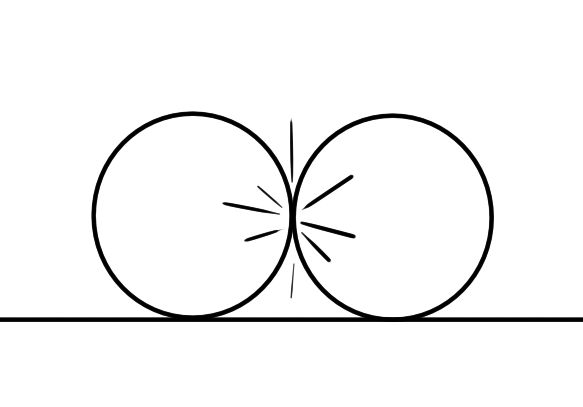
\includegraphics[width=0.8\textwidth]{images/1.jpg}

  \end{figure}




    \end{frame}
    
    
    %%%%%%%%%%%%%%%%%%%%%%%%%%%%%%%%%%%%%%%%%%%%%%%%%%%%%%%%%%%%%%%%%%%


%%%%%%%%%%%%%%%%%%%%%%%%%%%%%%%%%%%%%%%%%%%%%%%%%%%%%%%%%%%%%%%%%%%


\begin{frame}
    \begin{itemize}
        \item $\sum \vec{ F}=0\rightarrow\Delta \vec p =0$
        \pause
        \item What is $\sum \vec F$?
    \end{itemize}
    \pause
    
    
    \begin{figure}[h!]  
        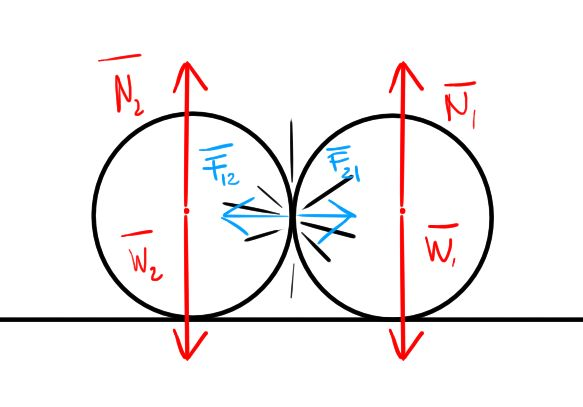
\includegraphics[width=0.8\textwidth]{images/2.jpg}
    
      \end{figure}
  
    
    
      \begin{itemize}
        \item $\sum \vec F=\vec N_1+\vec W_1+\vec N_2+\vec W_2+\vec F_{12}+\vec F_{21}=0\rightarrow \Delta p=0$
    \end{itemize}
    
    
    
        \end{frame}
        
  
%%%%%%%%%%%%%%%%%%%%%%%%%%%%%%%%%%%%%%%%%%%%%%%%%%%%%%%%%%%%%%%%%%%


\begin{frame}
    \begin{itemize}
        \item $\sum \vec{ F}=0\rightarrow\Delta \vec p =0$
        \pause
        \item What is $\sum \vec F$?
    \end{itemize}
    \pause
    
    
    \begin{figure}[h!]  
        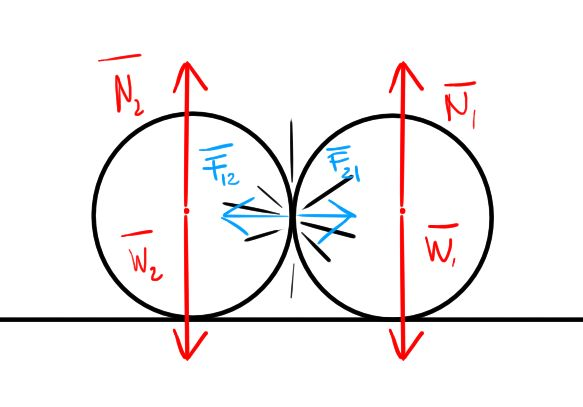
\includegraphics[width=0.6\textwidth]{images/2.jpg}
    
      \end{figure}
  
    
    
      \begin{itemize}
        \item $\sum \vec F_1=\vec N_1+\vec W_1+\vec F_{21}= \frac{\Delta \vec p_1}{\Delta t}$
 
        \item $\sum \vec F_2=\vec N_2+\vec W_2+\vec F_{21}= \frac{\Delta \vec p_2}{\Delta t}$
        \pause
        \item $\rightarrow \vec p_1=-\vec p_2$
    \end{itemize}
    
    
        \end{frame}
              
%%%%%%%%%%%%%%%%%%%%%%%%%%%%%%%%%%%%%%%%%%%%%%%%%%%%%%%%%%%%%%%%%%%


\begin{frame}

    
    \begin{figure}[h!]  
        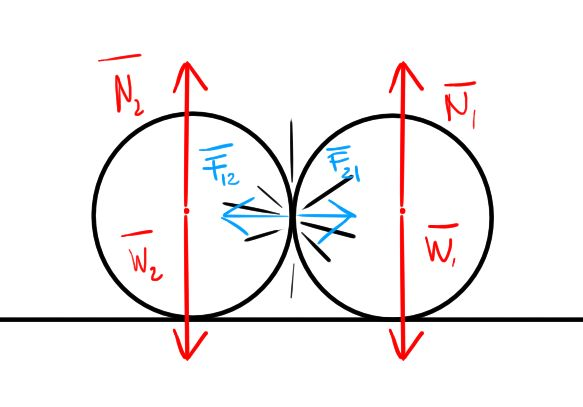
\includegraphics[width=0.7\textwidth]{images/2.jpg}
    
      \end{figure}
  
      If we consider the twoo balls as a system...
      \pause
   We define the linear momentum of the system to be,
   
   \begin{equation}
       \vec p=\vec p_1+\vec p_2
   \end{equation}
   \pause
      \begin{itemize}
        \item $\sum \vec F=\vec N_1+\vec W_1+\vec N_2+\vec W_2+\vec F_{12}+\vec F_{21}=0\rightarrow \Delta p=0$
    \end{itemize}
    
    
    
        \end{frame}

%%%%%%%%%%%%%%%%%%%%%%%%%%%%%%%%%%%%%%%%%%%%%%%%%%%%%%%%%%%%%%%%%%%


\begin{frame}

    \textbf{If the vector sum of the external forces on a system is zero, the total momentum
of the system is constant.}


\vspace{5mm}

Example: \url{https://www.youtube.com/watch?v=4IYDb6K5UF8}
    
        \end{frame}
        




        
        %%%%%%%%%%%%%%%%%%%%%%%%%%%%%%%%%%%%%%%%%%%%%%%%%%%%%%%%%%%%%%%%%%%

\begin{frame}
More than one particle?

\vspace{3mm}

\pause


  \begin{columns}[c]
    \column{2in}  % slides are 3in high by 5in wide
   
    \begin{figure}[h!]  
        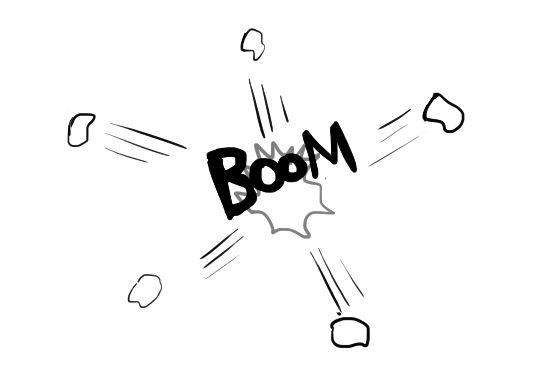
\includegraphics[width=1.\textwidth]{images/3.jpg}
      
      \end{figure}

      
    \column{2in}
 


    We define the total momentum as,

\begin{equation*}
    \vec p= \vec p_1+\vec p_2+\vec p_3+\vec p_4+\vec p_5
\end{equation*}

\pause
No external forces $\rightarrow \Delta \vec p=0$

\pause


\begin{equation*}
    \rightarrow \Delta \vec p_x= 0
\end{equation*}

\begin{equation*}
    \rightarrow \Delta \vec p_y= 0
\end{equation*}


    \end{columns}




  \end{frame}
                
                
%%%%%%%%%%%%%%%%%%%%%%%%%%%%%%%%%%%%%%%%%%%%%%%%%%%%%%%%%%%%%%%%%%%

        \begin{frame}
           External force...
            
 
            
            
              \begin{columns}[c]
                \column{2in}  % slides are 3in high by 5in wide
               
                \begin{figure}[h!]  
                    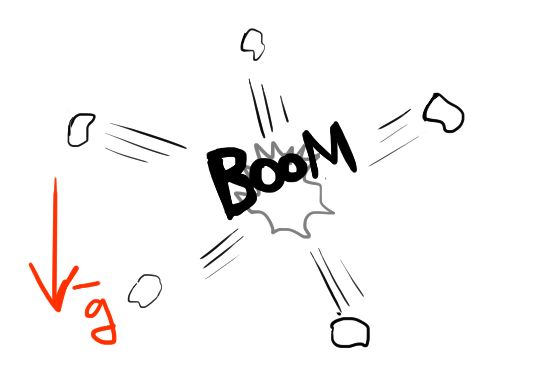
\includegraphics[width=1.\textwidth]{images/4.jpg}
                  
                  \end{figure}
            
                  
                \column{2in}
             
            
          
        
            
            
            \begin{equation*}
                \sum \vec F = \frac{\Delta \vec p}{\Delta t}
            \end{equation*}
            
            \begin{equation*}
                \rightarrow \Delta \vec p_x= F_x
            \end{equation*}
            
            \begin{equation*}
                \rightarrow \Delta \vec p_y= F_y
            \end{equation*}
            
   
            
        \end{columns}




              \end{frame}



                
%%%%%%%%%%%%%%%%%%%%%%%%%%%%%%%%%%%%%%%%%%%%%%%%%%%%%%%%%%%%%%%%%%%

\begin{frame}
    External force...
     

     
     
       \begin{columns}[c]
         \column{2in}  % slides are 3in high by 5in wide
        
         \begin{figure}[h!]  
             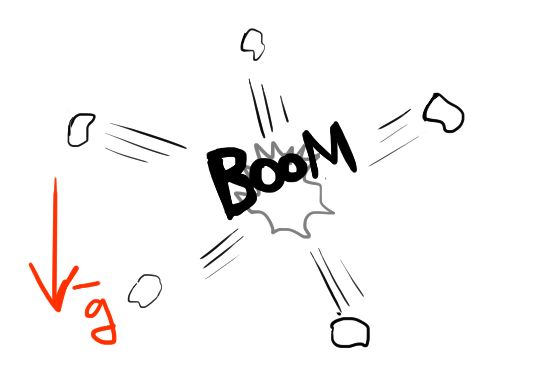
\includegraphics[width=1.\textwidth]{images/4.jpg}
           
           \end{figure}
     
           
         \column{2in}
      
     
   
 
     
     
     \begin{equation*}
         \sum \vec F = \frac{\Delta \vec p}{\Delta t}
     \end{equation*}
     
     \begin{equation*}
         \rightarrow \Delta \vec p_x= 0
     \end{equation*}
     
     \begin{equation*}
         \rightarrow \Delta \vec p_y= \sum_i m_i\vec g_i
     \end{equation*}
     

     
 \end{columns}




       \end{frame}


%%%%%%%%%%%%%%%%%%%%%%%%%%%%%%%%%%%%%%%%%%%%%%%%%%%%%%%%%%%%%%%%%%%

\begin{frame}
Example
\vspace{3mm}

A marksman holds a rifle of mass $m_R=3.00$ kg loosely, so it can
recoil freely. He fires a bullet of mass $m_B=5.00$ g horizontally
with a velocity relative to the ground of $v_{Bx}=300$ m/s. What is
the recoil velocity $v_{Rx}$ of the rifle? What are the final momentum
 of the bullet and rifle?



 \begin{figure}[h!]  
    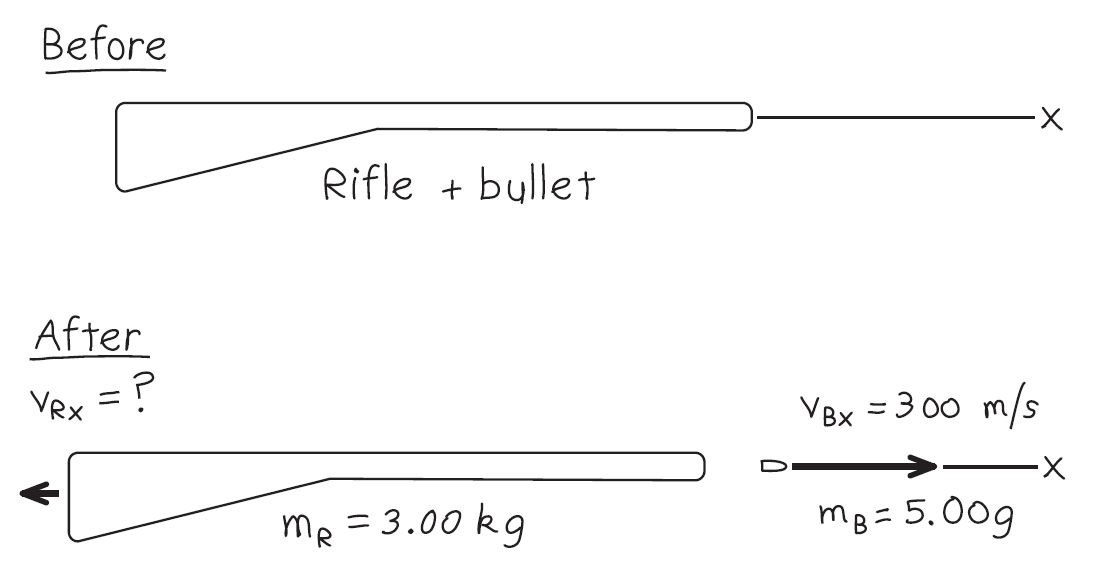
\includegraphics[width=0.7\textwidth]{images/5.jpg}
    \caption{ {\tiny Figures from Sears and Zemansky's University Physics 
    with Modern Physics, 13th Edition.} }
  \end{figure}


\end{frame}



%%%%%%%%%%%%%%%%%%%%%%%%%%%%%%%%%%%%%%%%%%%%%%%%%%%%%%%%%%%%%%%%%%%

\begin{frame}
    Example
    \vspace{3mm}
    
    Two gliders with different masses move toward each other on a
    frictionless air track. After they collide,
    glider $B$ has a final velocity of $+2.0$ m/s. What is the
    final velocity of glider $A$? How do the changes in momentum and
    in velocity compare?
    
    
    
     \begin{figure}[h!]  
        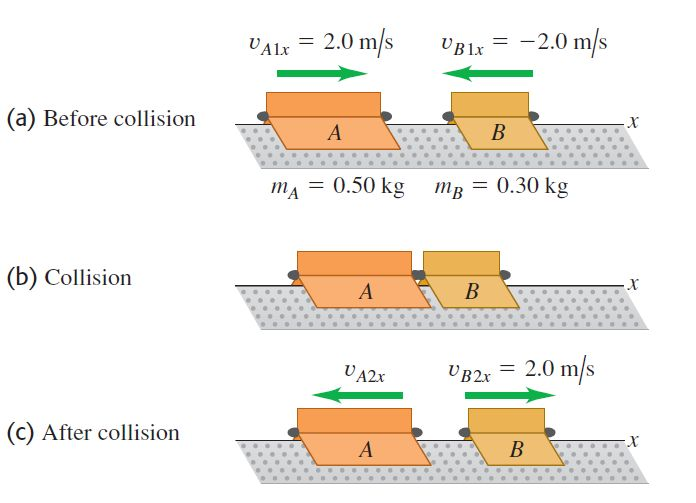
\includegraphics[width=0.7\textwidth]{images/6.jpg}
        \caption{ {\tiny Figures from Sears and Zemansky's University Physics 
        with Modern Physics, 13th Edition.} }
      \end{figure}
    
    
    \end{frame}




%%%%%%%%%%%%%%%%%%%%%%%%%%%%%%%%%%%%%%%%%%%%%%%%%%%%%%%%%%%%%%%%%%%

\begin{frame}
    Example
    \vspace{3mm}
    
Test Your Understanding
\vspace{3mm}

A spring-loaded toy sits at rest on a horizontal, frictionless surface. When the spring releases, the toy breaks
into three equal-mass pieces, $A$, $B$, and $C$, which slide along the surface. Piece $A$
moves off in the negative x-direction, while piece $B$ moves off in the negative y-direction.
\vspace{3mm}

\begin{enumerate}
    \item What are the signs of the velocity components of piece $C$?
    \item Which of the three pieces is moving the fastest?
\end{enumerate}



    
    
    \end{frame}


%%%%%%%%%%%%%%%%%%%%%%%%%%%%%%%%%%%%%%%%%%%%%%%%%%%%%%%%%%%%%%%%%%%

\begin{frame}
    Example
    \vspace{3mm}
    
Two kind of collisions
\vspace{3mm}

\begin{itemize}
    \item Elastic Collisions: the total kinetic energy of the system is the
    same after the collision as before (billiard balls).
    \item Inelastic Collisions: the total kinetic energy of the system is not conserved 
    (collision between 2 pieces of clay).
\end{itemize}



    
    
    \end{frame}


%%%%%%%%%%%%%%%%%%%%%%%%%%%%%%%%%%%%%%%%%%%%%%%%%%%%%%%%%%%%%%%%%%%

\begin{frame}
    Example
    \vspace{3mm}
    
Example: Collision with a wall



    
    
    \end{frame}


%%%%%%%%%%%%%%%%%%%%%%%%%%%%%%%%%%%%%%%%%%%%%%%%%%%%%%%%%%%%%%%%%%%

\begin{frame}
    Example
    \vspace{3mm}
    
Example of inelastic collision in 2D: An automobile collision
\vspace{3mm}


A $1000~kg$ car traveling north at collides with a $2000~kg$
truck traveling east at The occupants, wearing seat belts,
are uninjured, but the two vehicles move away from the impact
point as one. The insurance adjustor asks you to find the velocity
of the wreckage just after impact. What is your answer?

\begin{figure}[h!]  
    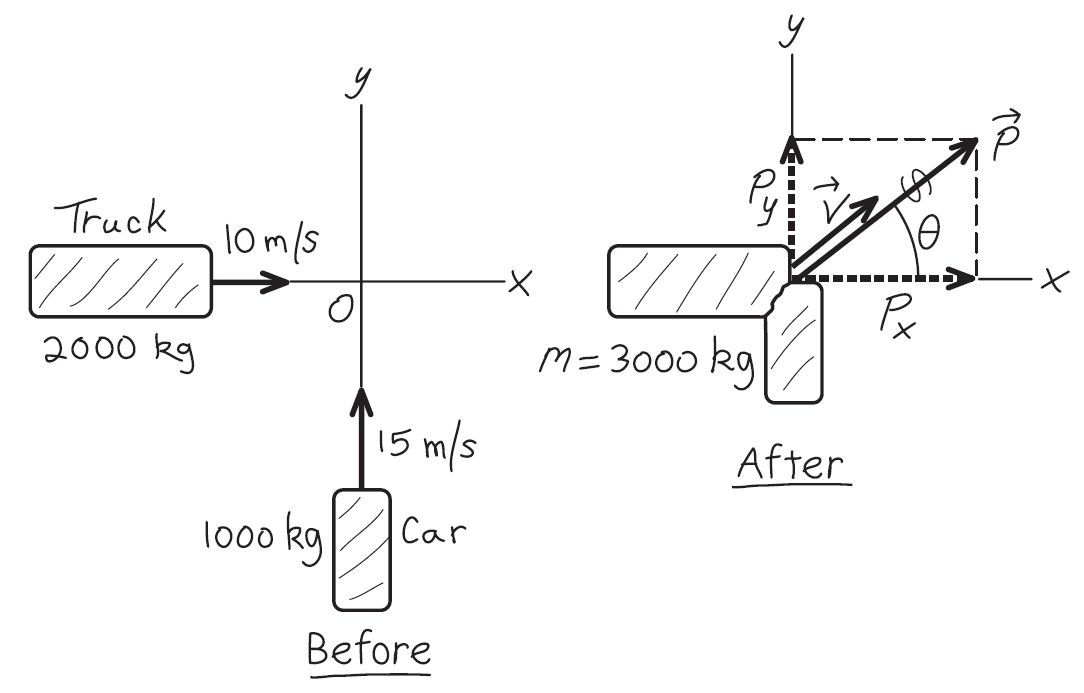
\includegraphics[width=0.7\textwidth]{images/7.jpg}
    \caption{ {\tiny Figures from Sears and Zemansky's University Physics 
    with Modern Physics, 13th Edition.} }
  \end{figure}

    
    
    \end{frame}

%%%%%%%%%%%%%%%%%%%%%%%%%%%%%%%%%%%%%%%%%%%%%%%%%%%%%%%%%%%%%%%%%%%

\begin{frame}

Testing you understanding about Linear Momentum.
\vspace{7mm}

(a) When a large car collides with a small car, which one undergoes
the greater change in momentum: the large one or the small
one? Or is it the same for both? (b) In light of your answer to part (a),
why are the occupants of the small car more likely to be hurt than
those of the large car, assuming that both cars are equally sturdy?

 \end{frame}
%%%%%%%%%%%%%%%%%%%%%%%%%%%%%%%%%%%%%%%%%%%%%%%%%%%%%%%%%%%%%%%%%%%

\begin{frame}

    Testing you understanding about Linear Momentum.
    \vspace{7mm}
    
 
    A woman holding a large rock stands on a frictionless, horizontal
sheet of ice. She throws the rock with speed $v_0$ at an angle
above the horizontal. Consider the system consisting of the woman
plus the rock. Is the momentum of the system conserved? Why or
why not? Is any component of the momentum of the system conserved?
Again, why or why not?
    
\vspace{7mm}

EXANPLE: \url{https://www.youtube.com/watch?v=Kf0bBxmNeec}
     \end{frame}


%%%%%%%%%%%%%%%%%%%%%%%%%%%%%%%%%%%%%%%%%%%%%%%%%%%%%%%%%%%%%%%%%%%

\begin{frame}

    Testing you understanding about Linear Momentum.
    \vspace{7mm}
    
 
    A glass dropped on the floor is more likely to break if the
    floor is concrete than if it is wood. Why?
    
     \end{frame}






%%%%%%%%%%%%%%%%%%%%%%%%%%%%%%%%%%%%%%%%%%%%%%%%%%%%%%%%%%%%%%%%%%%



\subsection{Center Of Mass}
\begin{frame}
   \textbf{CENTER OF MASS}
    \vspace{7mm}
    
    The total mass of the system is: $M=\sum_i m_i$
    \vspace{5mm}
  
    We define the \textbf{Center of Mass} of the system as,
  
    \begin{equation}
      \vec{R}=\frac{1}{M}\sum_i m_i \vec{r}_i
      \label{CM}
    \end{equation}
    
    
    \end{frame}







%%%%%%%%%%%%%%%%%%%%%%%%%%%%%%%%%%%%%%%%%%%%%%%%%%%%%%%%%%%%%%%%%%%


\begin{frame}
    \textbf{CENTER OF MASS}
     \vspace{7mm}
     
   EXAMPLE: Center of mass of a water molecule
     \vspace{5mm}
   
$d=9.57\times 10^{-11}$ m, $m_o=16~u$, $m_H=1~u$
     \begin{figure}[h!]  
        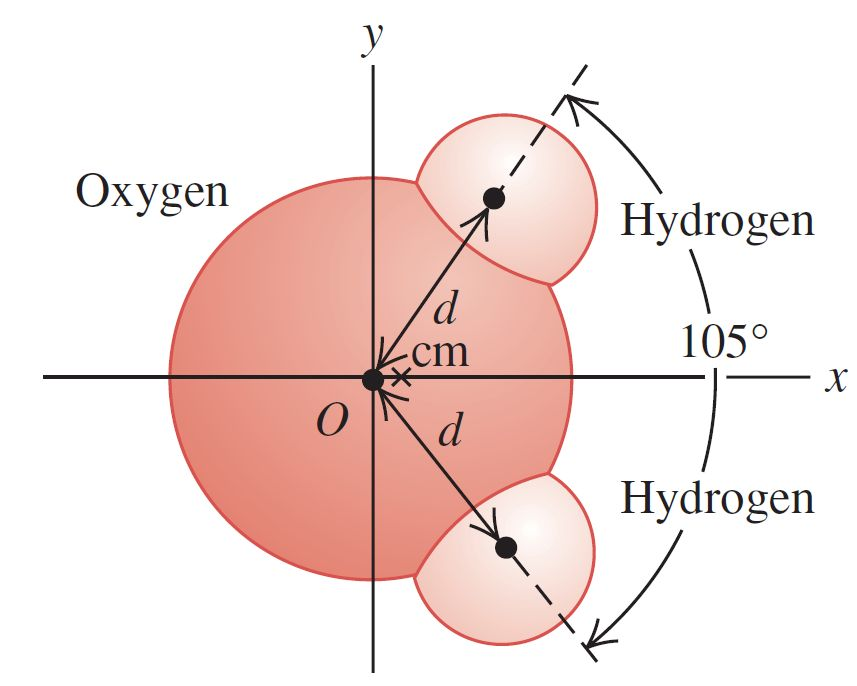
\includegraphics[width=0.6\textwidth]{images/8.jpg}
        \caption{ {\tiny Figures from Sears and Zemansky's University Physics 
        with Modern Physics, 13th Edition.} }
      \end{figure}
     
     
     \end{frame}
 

%%%%%%%%%%%%%%%%%%%%%%%%%%%%%%%%%%%%%%%%%%%%%%%%%%%%%%%%%%%%%%%%%%%

\begin{frame}
    \textbf{CENTER OF MASS}
     \vspace{7mm}

     
      \begin{columns}[c]
        \column{2in}  % slides are 3in high by 5in wide
       
           
     \begin{figure}[h!]  
        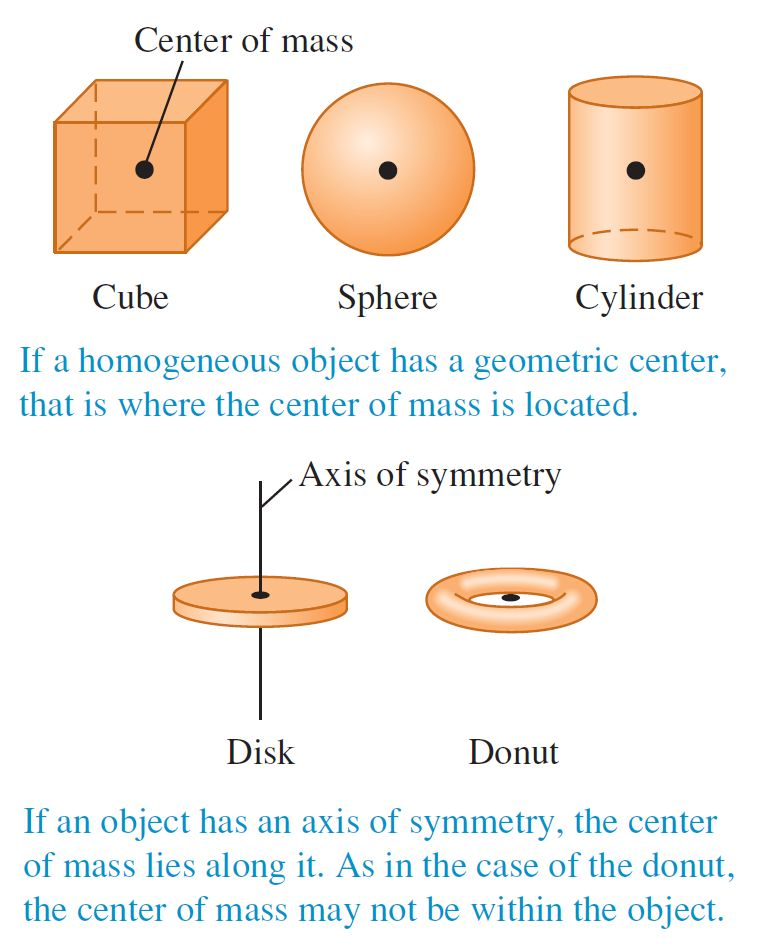
\includegraphics[width=0.7\textwidth]{images/9.jpg}
        \caption{ {\tiny Figures from Sears and Zemansky's University Physics 
        with Modern Physics, 13th Edition.} }
      \end{figure}

    
          
        \column{2in}
     
    
  

    
        For solid bodies, in which we have (at least on a macroscopic level) a continuous
        distribution of matter, the sums in eq. \ref{CM} have to be replaced by integrals.

    
\end{columns}




     \end{frame}





%%%%%%%%%%%%%%%%%%%%%%%%%%%%%%%%%%%%%%%%%%%%%%%%%%%%%%%%%%%%%%%%%%%

\begin{frame}
    \textbf{MOTION OF THE CENTER OF MASS}
     \vspace{7mm}

  We can show that,
  
  
  \begin{equation}
      \vec{P}=M\vec{V}_{CM}
  \end{equation}



  \begin{equation}
    \sum \vec{F}_{ext}=M\vec{a}_{CM}
\end{equation}




     \end{frame}








%%%%%%%%%%%%%%%%%%%%%%%%%%%%%%%%%%%%%%%%%%%%%%%%%%%%%%%%%%%%%%%%%%%

\begin{frame}
    \textbf{MOTION OF THE CENTER OF MASS}
     \vspace{7mm}




\textbf{When a body or a collection of particles is acted on by external forces, the center
of mass moves just as though all the mass were concentrated at that point and it
were acted on by a net force equal to the sum of the external forces on the system.}
\vspace{7mm}



     \end{frame}

 %%%%%%%%%%%%%%%%%%%%%%%%%%%%%%%%%%%%%%%%%%%%%%%%%%%%%%%%%%%%%%%%%%%

          \begin{frame}
            \begin{columns}[c]
                \column{2in}  % slides are 3in high by 5in wide
               
                   

            

This is a  very impressive result!!




            
                  
                \column{2in}
             
            
                \begin{figure}[h!]  
                    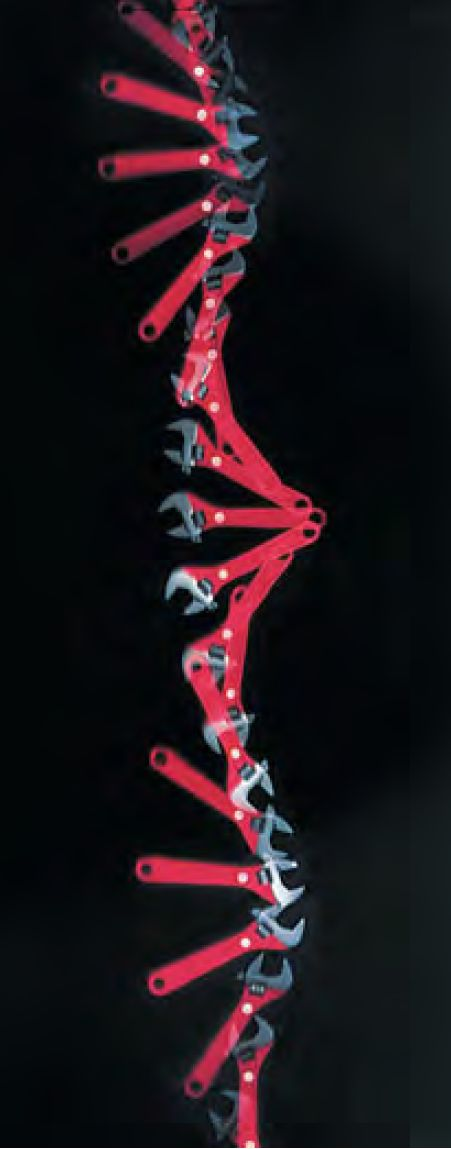
\includegraphics[width=0.7\textwidth]{images/11.jpg}
                    \caption{ {\tiny Figures from Sears and Zemansky's University Physics 
                    with Modern Physics, 13th Edition.} }
                  \end{figure}
            
          
        
            
        \end{columns}
        
             \end{frame}



     %%%%%%%%%%%%%%%%%%%%%%%%%%%%%%%%%%%%%%%%%%%%%%%%%%%%%%%%%%%%%%%%%%%

\begin{frame}
    \textbf{EXAMPLE}
     \vspace{7mm}


     \begin{figure}[h!]  
        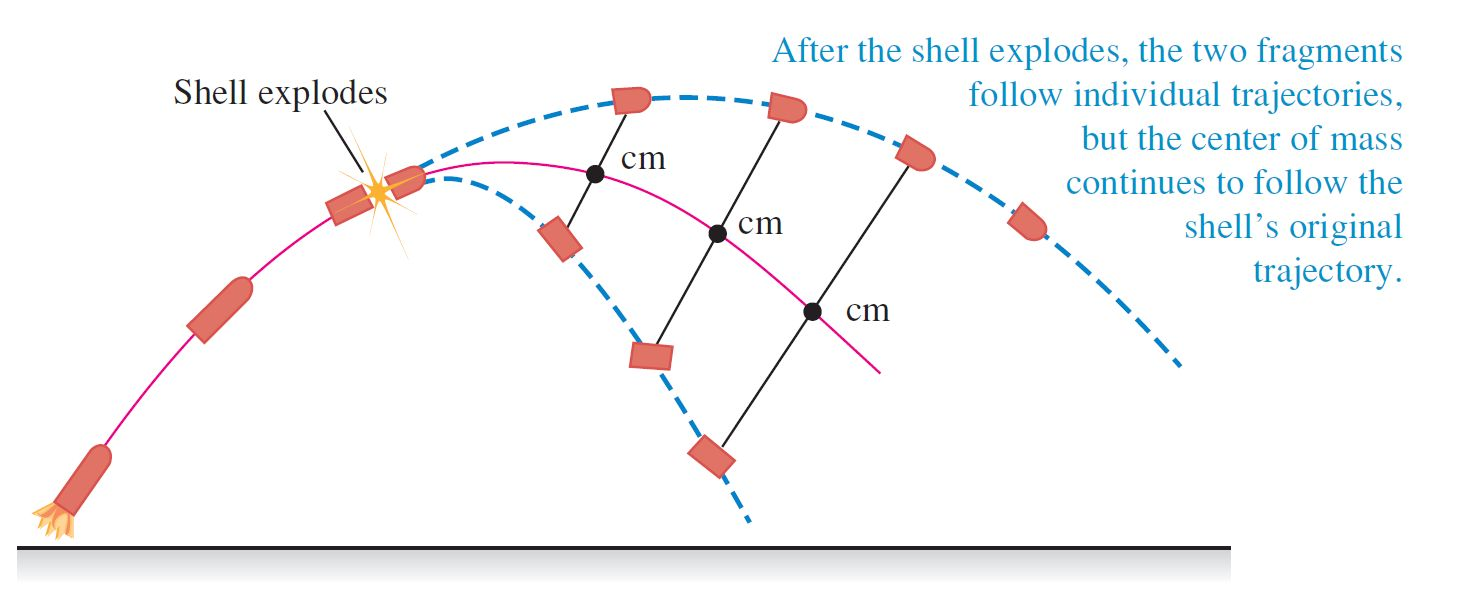
\includegraphics[width=0.8\textwidth]{images/10.jpg}
        \caption{ {\tiny Figures from Sears and Zemansky's University Physics 
        with Modern Physics, 13th Edition.} }
      \end{figure}

\pause
\vspace{7mm}


Will the center of mass in the figure
continue on the same parabolic trajectory even after one of the fragments hits the ground?
Why or why not?

     \end{frame}

%%%%%%%%%%%%%%%%%%%%%%%%%%%%%%%%%%%%%%%%%%%%%%%%%%%%%%%%%%%%%%%%%%%

\begin{frame}
    \textbf{EXAMPLE}
     \vspace{7mm}

    Explain the motion of a Newton Cradle
    
    \vspace{7mm}
        
    \url{https://www.youtube.com/watch?v=8dgyPRA86K0}
        
  \end{frame}

 %%%%%%%%%%%%%%%%%%%%%%%%%%%%%%%%%%%%%%%%%%%%%%%%%%%%%%%%%%%%%%%%%%%
\subsection{Rotation of Rigid Bodies}

\begin{frame}
    \textbf{Rotation of Rigid Bodies}
    \vspace{7mm}

     \begin{itemize}
         \item We are going to start studing motion of Rigid Bodies.
         \pause
         \item They are systems of particles with constant distance between them.
    \pause
         \item Macroscopically we see a continuous body.
         \pause 
         \item We can not represented adequately their motion as a moving point.
     \end{itemize}

     \end{frame}

     %%%%%%%%%%%%%%%%%%%%%%%%%%%%%%%%%%%%%%%%%%%%%%%%%%%%%%%%%%%%%%%%%%%

    
\begin{frame}
  

     We are going to represent the motion of rigid bodies as the superposition of two motions:
     \pause
     \begin{itemize}
    
         \item Translation of center of Mass + rotation around the Center of Mass.
         \pause
         \item We are going to consider only planar rotations, that is rotations in 2D (example: rotation of a wheel).
         \pause
         \item Rotations in 3D have a much more complex mechanics.
   

        \end{itemize}



     \end{frame}

     %%%%%%%%%%%%%%%%%%%%%%%%%%%%%%%%%%%%%%%%%%%%%%%%%%%%%%%%%%%%%%%%%%%

    
     \begin{frame}
   
    

      \begin{itemize}
          \item  To describe rotations, we need angles
          \pause
          \item We are going to use $\theta$, $\omega$ and $\alpha$
          \pause
          \item Till now, we have been using just numbers to represent them,

      \end{itemize}
    
      \begin{equation*}
        \omega = \frac{\Delta \theta}{\Delta t},\ \alpha=\frac{\Delta \omega}{\Delta t} \ (\alpha \ constant)
      \end{equation*}

       \pause


       \begin{itemize}
        \item  But rotations can have two different sense, so to specify a rotation, we need a numbersand a
         sense.
         \item Angular velocity and Acceleration are represented by vectors!

    \end{itemize}

         \end{frame}
    
%%%%%%%%%%%%%%%%%%%%%%%%%%%%%%%%%%%%%%%%%%%%%%%%%%%%%%%%%%%%%%%%%%%

         \begin{frame}
     
        
    

    
         \begin{figure}[h!]  
            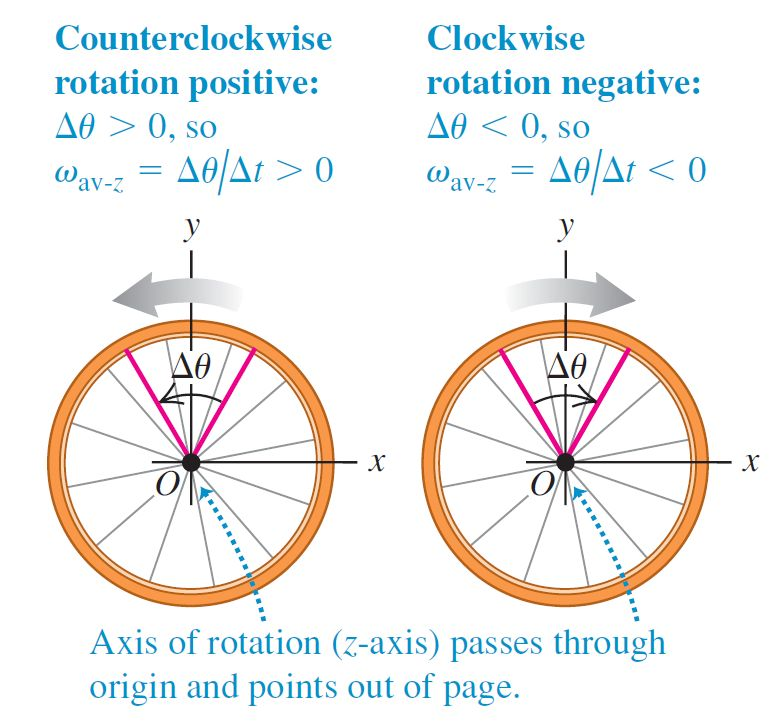
\includegraphics[width=0.6\textwidth]{images/12.jpg}
            \caption{ {\tiny Figures from Sears and Zemansky's University Physics 
            with Modern Physics, 13th Edition.} }
          \end{figure}
    
    
        
        
             \end{frame}
        


%%%%%%%%%%%%%%%%%%%%%%%%%%%%%%%%%%%%%%%%%%%%%%%%%%%%%%%%%%%%%%%%%%%

\begin{frame}
     
     \textbf{Angular Velocity As a Vector}   
     \vspace{3mm}
    

     \begin{figure}[h!]  
        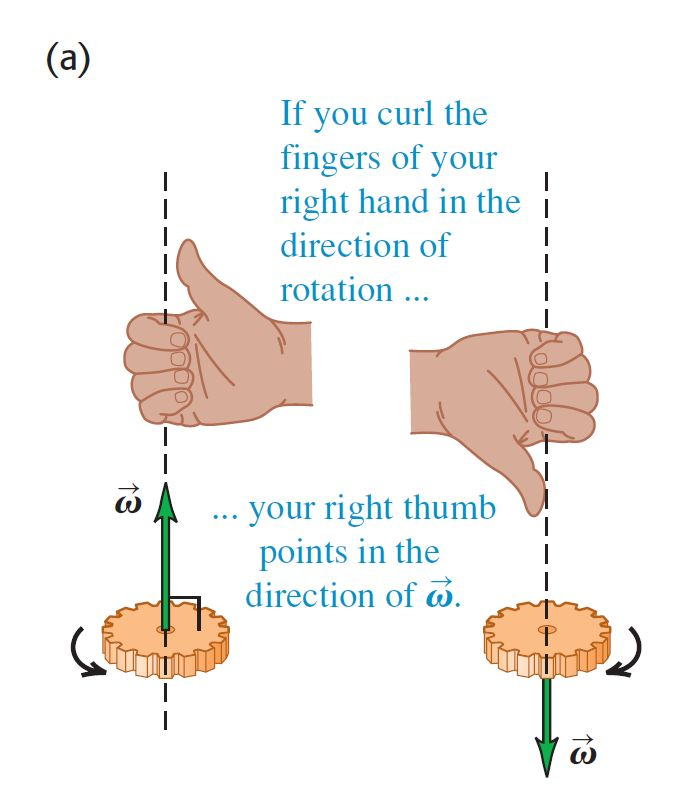
\includegraphics[width=0.6\textwidth]{images/13.jpg}
        \caption{ {\tiny Figures from Sears and Zemansky's University Physics 
        with Modern Physics, 13th Edition.} }
      \end{figure}
   
   
        \end{frame}
   
%%%%%%%%%%%%%%%%%%%%%%%%%%%%%%%%%%%%%%%%%%%%%%%%%%%%%%%%%%%%%%%%%%%

\begin{frame}
     
    \textbf{Angular Acceleration As a Vector}   
    \vspace{3mm}
   

    \begin{figure}[h!]  
       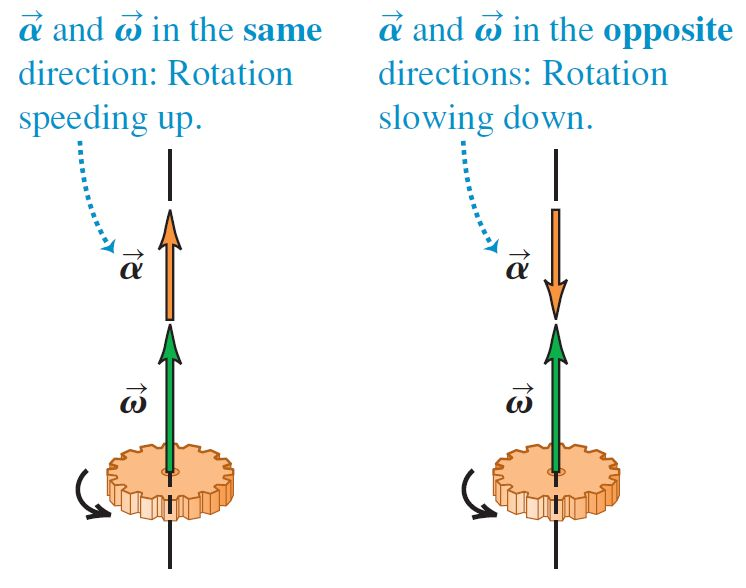
\includegraphics[width=0.6\textwidth]{images/14.jpg}
       \caption{ {\tiny Figures from Sears and Zemansky's University Physics 
       with Modern Physics, 13th Edition.} }
     \end{figure}
  
  
       \end{frame}
  

%%%%%%%%%%%%%%%%%%%%%%%%%%%%%%%%%%%%%%%%%%%%%%%%%%%%%%%%%%%%%%%%%%%

\begin{frame}
     
    Test Your Understanding 
    \vspace{3mm}
    The figure shows a graph of $\omega_z$ and $\alpha_z$ versus time
    for a particular rotating body. (a) During which time
    intervals is the rotation speeding up?

    \begin{figure}[h!]  
       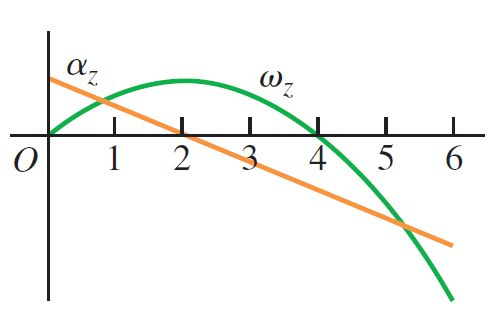
\includegraphics[width=0.6\textwidth]{images/15.jpg}
       \caption{ {\tiny Figures from Sears and Zemansky's University Physics 
       with Modern Physics, 13th Edition.} }
     \end{figure}
  
  
       \end{frame}
  
%%%%%%%%%%%%%%%%%%%%%%%%%%%%%%%%%%%%%%%%%%%%%%%%%%%%%%%%%%%%%%%%%%%

\begin{frame}
  \textbf{Comparison of Linear and Angular Motion with
  Constant Acceleration}   
  \vspace{5mm}

  \begin{figure}[h!]  
    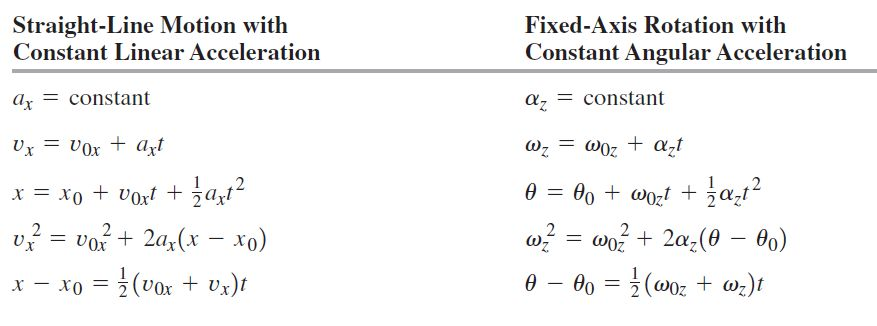
\includegraphics[width=1.0\textwidth]{images/16.jpg}
    \caption{ {\tiny Table from Sears and Zemansky's University Physics 
    with Modern Physics, 13th Edition.} }
  \end{figure}
  
       \end{frame}
  



%%%%%%%%%%%%%%%%%%%%%%%%%%%%%%%%%%%%%%%%%%%%%%%%%%%%%%%%%%%%%%%%%%%

\begin{frame}
    \textbf{Rotation with constant angular acceleration}   
    \vspace{5mm}


    

      
      


      
   \begin{columns}[c]
    \column{2in}  % slides are 3in high by 5in wide
   


    You have finished watching a movie on Blu-ray and the disc is
    slowing to a stop. The disc’s angular velocity at $t=0$ is $27.5~rad/s$,
    and its angular acceleration is a constant $-10~rad/s^2$. A line $PQ$
    on the disc’s surface lies along the at $t=0$.
    (a) What is the disc’s angular velocity at $t=0.3~s$ (b) What
    angle does the line $PQ$ make with the $+x-axis$ at this time?
    



    \column{2in}
 

    \begin{figure}[h!]  
        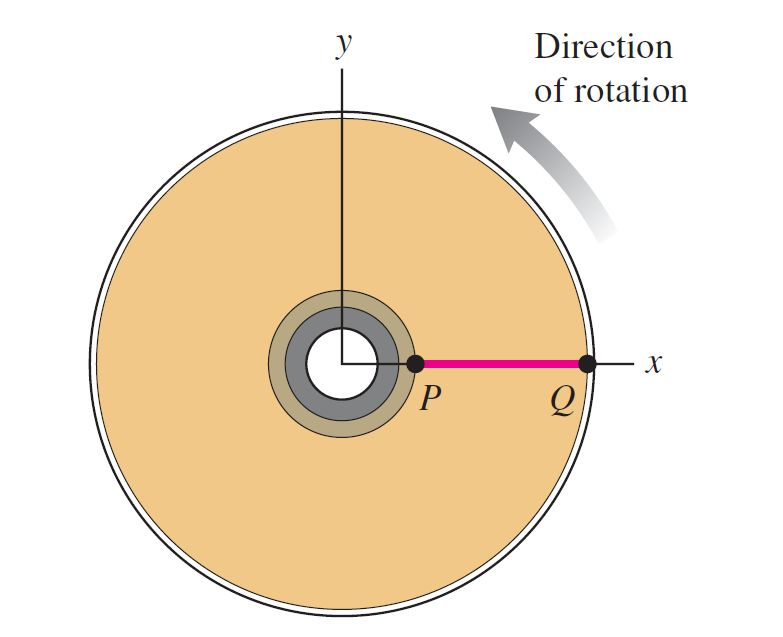
\includegraphics[width=0.8\textwidth]{images/18.jpg}
        \caption{ {\tiny Table from Sears and Zemansky's University Physics 
        with Modern Physics, 13th Edition.} }
        \label{disc}
      \end{figure}


    \end{columns}





    \end{frame}

%%%%%%%%%%%%%%%%%%%%%%%%%%%%%%%%%%%%%%%%%%%%%%%%%%%%%%%%%%%%%%%%%%%

\begin{frame}
    \textbf{Relating Linear and Angular Kinematics}   
    \vspace{5mm}
  
\begin{equation*}
    \boxed{v=r\omega, \ a_{rad}=\omega^ 2r}  
\end{equation*}
    
         \end{frame}
    
  %%%%%%%%%%%%%%%%%%%%%%%%%%%%%%%%%%%%%%%%%%%%%%%%%%%%%%%%%%%%%%%%%%%



  \begin{frame}
    \textbf{Relating Linear and Angular Kinematics}   
    \vspace{5mm}
  
\begin{equation*}
    \boxed { v=r\omega, \ a_{rad}=\omega^ 2r, \ \textcolor{blue}{ a_{tan}=r\alpha}}
\end{equation*}
    
         \end{frame}
    
  %%%%%%%%%%%%%%%%%%%%%%%%%%%%%%%%%%%%%%%%%%%%%%%%%%%%%%%%%%%%%%%%%%%


  \begin{frame}
    \textbf{Throwing a discus}   
    \vspace{5mm}
  
    An athlete whirls a discus in a circle of radius $80.0 cm$. At a certain
    instant, the athlete is rotating at $10~rad/s$ and the angular speed
    is increasing at $50~rad/s^2$. At this instant, find the tangential and
    centripetal components of the acceleration of the discus and the
    magnitude of the acceleration.
    



    \vspace{5mm}

    \begin{figure}[h!]  
      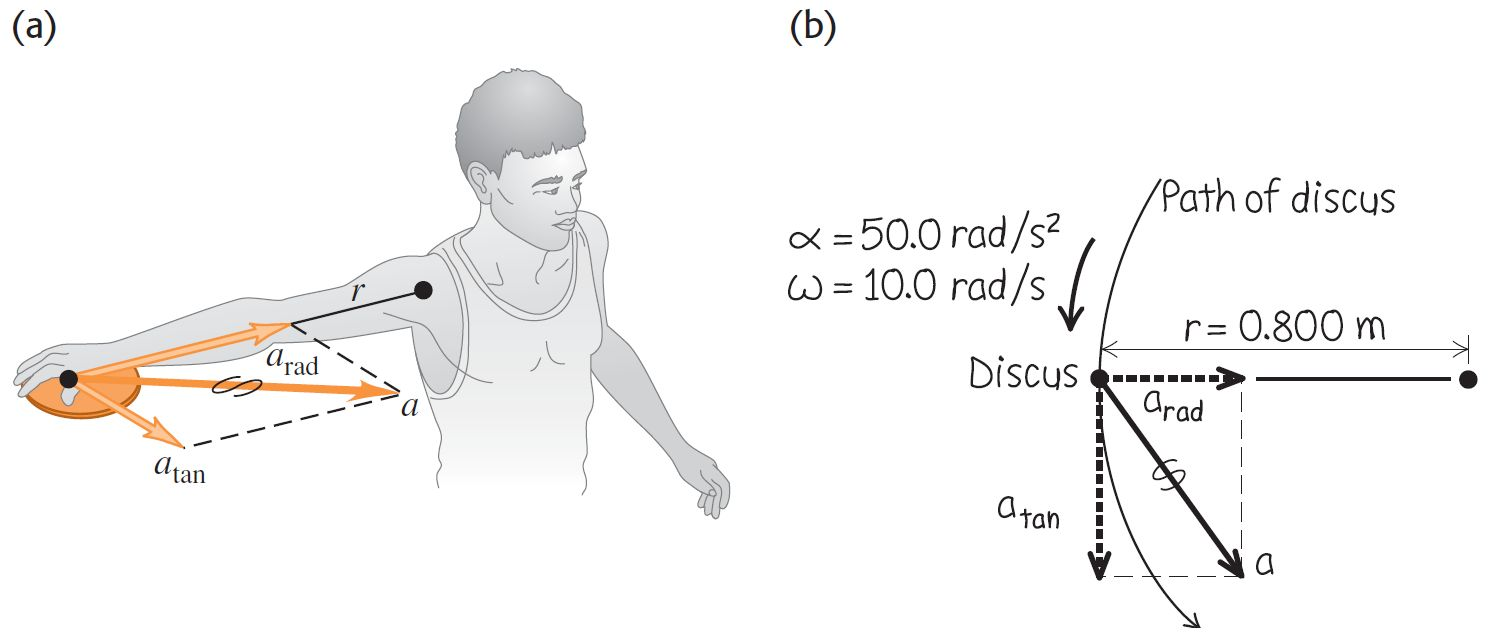
\includegraphics[width=1.0\textwidth]{images/17.jpg}
      \caption{ {\tiny Figure from Sears and Zemansky's University Physics 
      with Modern Physics, 13th Edition.} }
    \end{figure}




         \end{frame}
    
  %%%%%%%%%%%%%%%%%%%%%%%%%%%%%%%%%%%%%%%%%%%%%%%%%%%%%%%%%%%%%%%%%%%



  \begin{frame}
    \textbf{Throwing a discus}   
    \vspace{5mm}


 Information is stored on a
  disc (see Fig. \ref{disc}) in a coded pattern of tiny pits. The pits are arranged in a track
  that spirals outward toward the rim of the disc. As the disc spins inside a player,
  the track is scanned at a constant linear speed. How must the rotation speed of the disc
  change as the player’s scanning head moves over the track? (i) The rotation speed must
  increase. (ii) The rotation speed must decrease. (iii) The rotation speed must stay the
  same.





\end{frame}

    
  %%%%%%%%%%%%%%%%%%%%%%%%%%%%%%%%%%%%%%%%%%%%%%%%%%%%%%%%%%%%%%%%%%%









%%%%%%%%%%%%%%%%%%%%%%%%%%%%%%%%%%%%%%%%%%%%%%%%%%%%%%%%%%%%%%%%%%%
 \end{document}
%%%%%%%%%%%%%%%%%%%%%%%%%%%%%%%%%%%%%%%%%%%%%%%%%%%%%%%%%%%%%%%%%%%